\documentclass[tikz,border=10pt]{standalone}
\usepackage{tikz}
\usetikzlibrary{shapes,arrows,positioning,calc}

\begin{document}
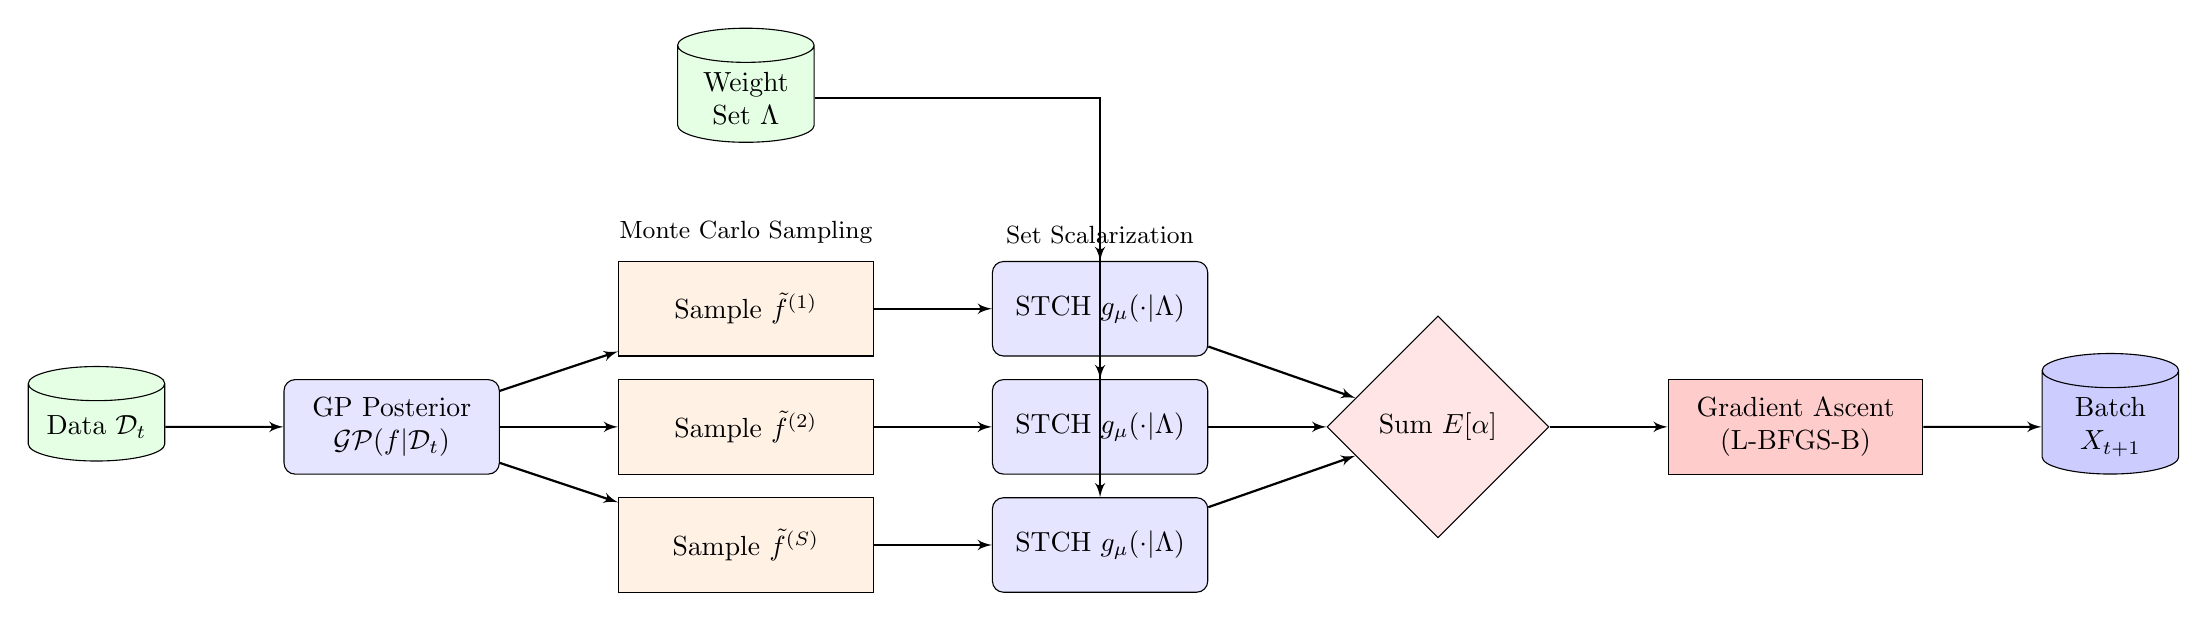
\begin{tikzpicture}[auto, node distance=1.5cm, >=latex']

    % Styles
    \tikzstyle{block} = [draw, rectangle, fill=blue!10, text width=2.5cm, text centered, minimum height=1.2cm, rounded corners]
    \tikzstyle{data} = [draw, cylinder, shape border rotate=90, aspect=0.25, fill=green!10, text width=1.5cm, text centered, minimum height=1.2cm]
    \tikzstyle{process} = [draw, rectangle, fill=orange!10, text width=3cm, text centered, minimum height=1.2cm]
    \tikzstyle{decision} = [draw, diamond, fill=red!10, text width=2cm, text centered]
    \tikzstyle{line} = [draw, ->, thick]

    % Nodes
    \node [data] (data) {Data $\mathcal{D}_t$};
    \node [block, right=of data] (gp) {GP Posterior $\mathcal{GP}(f|\mathcal{D}_t)$};
    
    % Sampling block
    \node [process, right=of gp, yshift=1.5cm] (sample1) {Sample $\tilde{f}^{(1)}$};
    \node [process, right=of gp] (sample2) {Sample $\tilde{f}^{(2)}$};
    \node [process, right=of gp, yshift=-1.5cm] (sample3) {Sample $\tilde{f}^{(S)}$};
    
    % Weights
    \node [data, above=of sample1] (weights) {Weight Set $\Lambda$};

    % Scalarization
    \node [block, right=of sample1] (stch1) {STCH $g_\mu(\cdot|\Lambda)$};
    \node [block, right=of sample2] (stch2) {STCH $g_\mu(\cdot|\Lambda)$};
    \node [block, right=of sample3] (stch3) {STCH $g_\mu(\cdot|\Lambda)$};

    % Aggregation
    \node [decision, right=of stch2] (sum) {Sum $\mathbb{E}[\alpha]$};
    
    % Optimization
    \node [process, right=of sum, fill=red!20] (opt) {Gradient Ascent (L-BFGS-B)};
    
    % Output
    \node [data, right=of opt, fill=blue!20] (batch) {Batch $X_{t+1}$};

    % Edges
    \path [line] (data) -- (gp);
    \path [line] (gp) -- (sample1);
    \path [line] (gp) -- (sample2);
    \path [line] (gp) -- (sample3);
    
    \path [line] (weights) -| (stch1);
    \path [line] (weights) -| (stch2);
    \path [line] (weights) -| (stch3);
    
    \path [line] (sample1) -- (stch1);
    \path [line] (sample2) -- (stch2);
    \path [line] (sample3) -- (stch3);
    
    \path [line] (stch1) -- (sum);
    \path [line] (stch2) -- (sum);
    \path [line] (stch3) -- (sum);
    
    \path [line] (sum) -- (opt);
    \path [line] (opt) -- (batch);

    % Labels
    \node [above=0.1cm of sample1] (mc) {\small Monte Carlo Sampling};
    \node [above=0.1cm of stch1] (sc) {\small Set Scalarization};

\end{tikzpicture}
\end{document}
